\chapter{Air- and Rail-Transport}
\label{ch:air}
% ##################################################################################################################

\hfill \textbf{Author:} Dominik Grether

\begin{center} 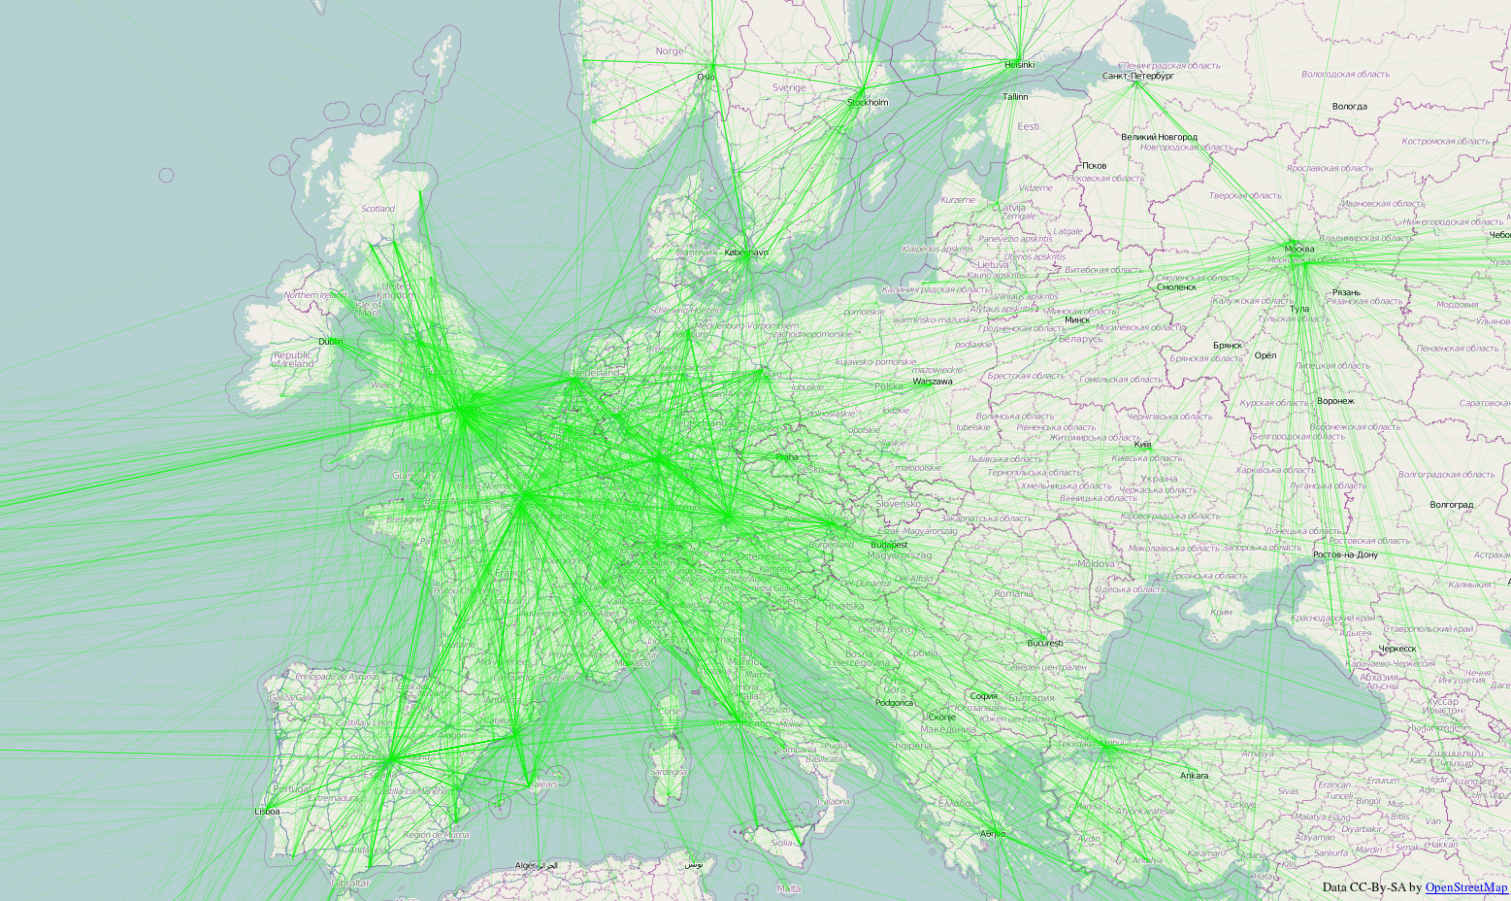
\includegraphics[width=0.25\textwidth, angle=0]{extending/figures/air/air_network_europe_osm} \end{center}

% ##################################################################################################################
%\section{Mid-Distance Transport}

Options for the simulation of air- and rail-transport technology and passengers using MATSim are subject of this chapter. 
Overall travel times are often not that different between middle range rail on one side, and air transportation on the other.
Airports and railway stations are affected by capacity and opening time constraints. 
For passengers and goods, their geospatial location is an important property. 
Both modes, but especially air transport, are faced with hard capacity restrictions. 

This chapter presents an approach how MATSim can be applied to capture these constraints and how the interaction between a passenger demand and the constraints on the technology supply can be modeled. 
The public transit model of MATSim (Chapter~\ref{ch:pt}) is applied. %public transit vehicles and stops. 
Airports and aircraft are microscopically modeled the same way as bus stops and buses. 
Passengers are represented microscopically as multi-agent demand for air transportation. 
Their choice of transport mode, routes, and departure time is restricted by the capacity provided by the simulation model for air transport technology. 
The modeling of rail transport is based on teleportation. 
With appropriate data the modeling approach for air transport could also be applied to rail transport~\citep{Quick2012BARailTraffic}.  

The modeling of technology and demand is sketched in Section~\ref{sec:air_rail_scenario}. 
Based on simulation results for a pure air transport model, effects of mode choice are presented (Section~\ref{sec:air_rail_results}). 
Section~\ref{sec:air_rail_discussion} then interprets simulation results and highlights some modeling aspects that require further studies. 
Especially the choice set generation and plans removal algorithm of MATSim is discussed, that is also subject of Section~\ref{sec:future-of-scoring-function}. 
Modeling, results, and studies of this chapter present the highlights of \citet[][Chapter~6, pp.~119]{Grether2014PhD} where further details can be found in case of interest.   

%\mnote{Rail \& Air Transport}
%In Italy, a private company started providing $2.5 \, h$ non-stop train rides between Milano and Rome\footnote{\url{http://www.italotreno.it} last access 19.12.2012}. 
%From Paris, nearly all major French cities can be reached by high-speed train in $2$--$4 \, h$ trips\footnote{\url{www.tgv-europe.com/en/}, last access 11.09.2012}. 
%For the journey Berlin--Frankfurt in Germany, a $4 \, h$ non-stop rail connection is provided\footnote{\url{www.bahn.com}, last access 11.09.2012}. 
%%
%Many airlines provide flights between all these destinations that take between $1$ and $2 \, h$.
%When comparing travel times, the additional access time to the airport or railway railway station needs to be included.
%Overall travel times are often not that different between middle range rail on one side, and air transportation on the other.
%
%\mnote{Airport Capacity}
%Following recent forecasts, in 2030, 13 major EU airports will operate at least eight hours at full capacity a day~\citep{EC2011COM823AirportPolicyEU}.
%Legal opening hour constraints limit operations to a certain time frame.
%Yet even increasing opening hours for airports may not resolve capacity bottlenecks, since it may not be possible to move enough demand away from the peak hours.
%
%\mnote{Location \& Time}
%In contrast, 
%railway stations are normally not as much exposed to restrictions of opening hours due to noise protection as airports are.
%Also, in comparison with airports, railway stations mostly feature a more central geospatial location in urban areas.
%Slightly longer 
%travel times can be compensated for by shorter access times and longer opening hours.
%Passenger demand and technology supply for mid-distance railway or air transportation may interact and are time dependent over a day or even a longer period. 
%
%\mnote{Infrastructure Planning}
%To provide more capacity, railway or air transport networks may be target of planned extensions. 
%New infrastructure is 
%often accompanied by new emissions of noise and pollutants and 
%is, thus, subject to lengthy planning, negotiation, and high private and public costs~\citep{BubaloDaduna2012AirportCapacityDemandSimmodBBI}.
%However, improvements on infrastructure may improve quality of journeys or offer even new possibilities of transportation. 
%Identification and appraisal of these disadvantages and benefits is one of the key subjects in infrastructure planning. 
%
%
%\mnote{Microscopic Assessment Model}
%Mutual reactions on several scales may arise if one or several transport measures cause positive or negative benefits for certain travelers. 
%For each transport system user, changes in price, travel times, schedule, or 
%available transport modes may have different impacts, which depend on planned activities, available budget and geospatial location. 
%
%
%% ################################################################################################################
%
%
%\mnote{Models for Air Transport Systems}
%For a review of simulation models for air transport system, see~\citep[e.g.~][pp.~121]{Grether2014PhD}. 
%
%In contrast, \citet{ClarkeEtAl2007AirNetworkSim} propose an event-based simulation approach, MEANSMIT, that targets at the simulation of air traffic flow management concepts, airline scheduling and strategic planning. 
%Passengers are explicitly included, but only during their journey. 
%The representation of passengers enables a detailed modelling of (de-)boarding, connection flight availability, and decision making when flights shall be cancelled. 
%MEANSMIT uses a queue model to simulate aircraft movement. 
%
%\mnote{Queue Models}
%Queueing theory and queue models are widely used to model the technology of air transportation systems.
%For example, \citet{PyrgiotisMaloneOdoni2011AirTrafficDelayPropagation} use queueing theory to model the propagation of delay through the network. 
%Effects of new airspace management technologies are studied by \citet{NikolerisHansen2012QueueingModelsAircraftOperations}.
%
%\mnote{Chosen Approach}
%As queue models seem to be well suited to model air transport systems, this work applies the queue model explained in Sec.~\ref{sec:gawron_extension} in the context of traffic signal control. 
%% for simulation of traffic flow.  
%The model provides several parameters for an explicitly modeled segment of a transport network: The maximum flow that can pass a segment, the maximum amount of vehicles on the segment, and a maximum velocity per segment or vehicle.  
%Several segments can be connected, building a transport network, on which individual vehicles can be simulated.  
%Segments are modeled as FIFO (first-in first-out) queues, nodes can be interpreted as servers.  
%Thus, the modeling of the road network is quite similar to queueing theory approaches in air transport \citep[e.g.][]{PyrgiotisMaloneOdoni2011AirTrafficDelayPropagation}.
%However, the proposed model is not solved analytically but by simulation.  
%While analytical solvable models may conserve computational resources, a computational fast simulation model enables an agent-based modeling of every individual throughout the complete simulation lifecycle in complex scenarios.
%For the technology side of air transport systems, the approach is quite similar to the approach chosen in MEANS---MIT~\citep{ClarkeEtAl2007AirNetworkSim}. 
%It is, however, more detailed in respect to the passenger model.  

% ##################################################################################################################
\section{Air Transport Scenario}
\label{sec:air_rail_scenario}

\subsection{Modeling \& Simulation of Air Transport Technology}
\label{sec:modeling-of-technology}

%\mnote{Overview}
%This section focusses on the technology side of air transport networks. 
%First, available data sources are reviewed. 
%Then, it is shown how airports and aircraft can be modeled microscopically by a queue model based network representation and a simulation approach for urban transport systems.
%At the end of the section simulation studies are presented that show how the model can represent runway capacity and delay. 

%show how the model works and how it can be enriched.

%\subsection{Data Sources}
%\label{sec:supply_data_sources}

%\mnote{OAG}
The air traffic technology model takes advantage of data provided by OAG Aviation\footnote{\url{www.oagaviation.com}, last access 08.08.2012}. 
%Details in \citet[][pp.~122]{Grether2014PhD}. 
%%An OAG snapshot of worldwide direct flights in September 2009 is available for schedule generation. 
%%All flights with IATA\footnote{see \url{www.iata.org}, last access 17.11.2013} airport codes, flight times, flight numbers and designators, aircraft types, available seats, and distance between airport are gathered from the database and processed. Codeshares, multi-stop flights, buses and trains with flight numbers, and cargo flights are filtered out of the schedule during the generation process.
Relevant data for schedule and network generation is excerpted from the September 2009 OAG data using all flights departing on a Tuesday, taking each specific flight number into account only once.
This may not always result in complete flight cycles, e.g.,\,when the outbound and inbound flight operate on different days of the week. 
Compared to using all flights of an entire week, the network may be incomplete, as certain destinations are only served on specific days.

%\mnote{Airport Capacity}
%Airport capacity data is available from many sources. 
%Read~\citet[][pp.~122]{Grether2014PhD} for a review of potential  data sources and usage,  

%\mnote{Airport Capacity}
%Airport capacity data is available from many sources.  
%However, no machine-readable source was found. Thus, the 
%50 busiest European airports in terms of total passengers per year were taken from wikipedia\footnote{\url{en.wikipedia.org/wiki/List_of_the_busiest_airports_in_Europe}, last access 05.08.2012},
%and data for those airports was researched manually.  
%A list of airport capacity information is given in Appendix~\ref{appendix:airport_capacity}, together with the source for each information item.  The list provides separate capacities for departures and arrivals.  All remaining airports are modeled with arrival and departure capacities of 60~aircraft per hour each.  This is considerably more capacity than what these airports provide in reality. 

\begin{figure}[t]
	\begin{minipage}{0.5\linewidth}
				\centering
			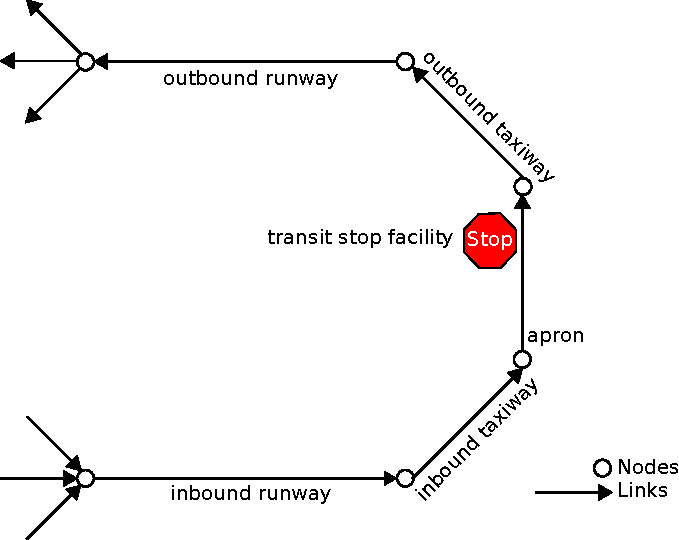
\includegraphics[width=0.9\textwidth]{extending/figures/air/sf_flight_model_airport.pdf}
		\vspace{1.3cm}

			%\scriptsize
			\footnotesize
			\begin{tabular}{@{}lrrr@{}}
				Linktype & Count & Length [m] & Speed [km/h] \\
				\hline
				Runway   	& 2					& 1500		& $length \cdot c_{flow} $  	\\ % former value 220
				Taxiway   	& 2					& 500		& 20  	\\
				Apron   		& 1					& 500		& 20  	\\
				\end{tabular}		
				\vspace{1.4cm}
				\caption{Airport layout and characteristics}
				\label{fig:matsim_airport}
	\end{minipage}
	\begin{minipage}{0.5\linewidth}
		\centering
		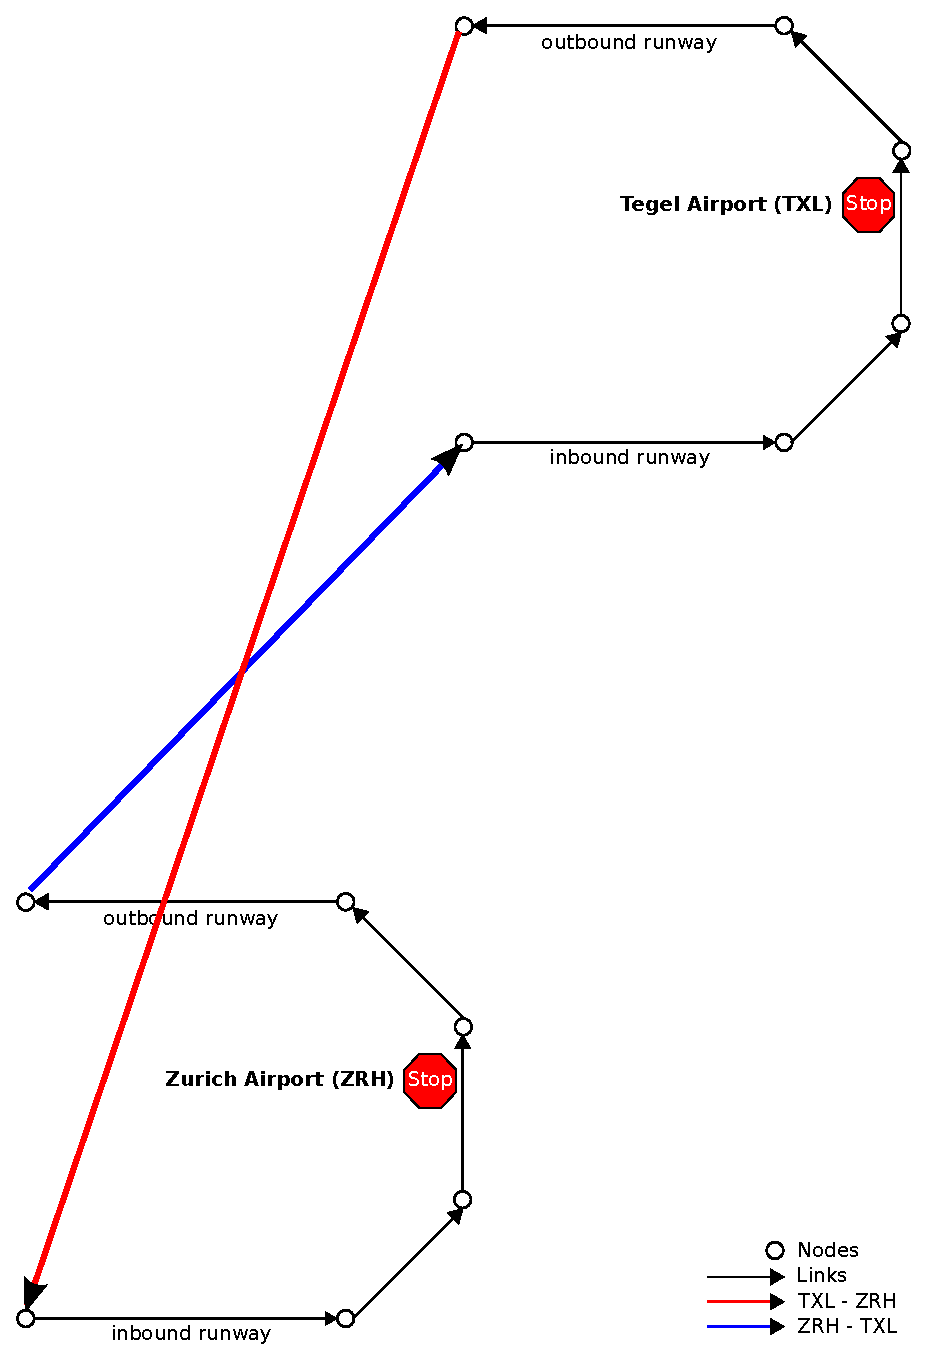
\includegraphics[width=0.9\textwidth]{extending/figures/air/sf_airport_network_no_slide.pdf}
		\caption{Network layout}
		\label{fig:matsim_network_model}
	\end{minipage}
  \caption{Layout of the air network}
	\label{fig:air_network}
\end{figure}

%\mnote{Network}
The modeling of the air network aims at a simulation by MATSim. %the queue model reviewed and explained in Sec.~\ref{sec:gawron_extension}. 
The network consists of airports, each showing an identical layout, and point-to-point connections in between. 
Every runway is solely used either for inbound or outbound flights with taxiways connecting the runways to the apron. The latter accommodates a transit stop, i.e., the terminal, where flight movements originate and terminate (Figure~\ref{fig:matsim_airport}). 
%\mnote{Runways}
%The two runways of each airport possess a restriction of flow capacity ($c_{flow}$) that is varied in the subsequent simulation runs. 
%Furthermore, not more than one aircraft (unit [$veh$]) can be simultaneously on a runway.
%This is modeled by setting the $c_{storage}$ parameter of the queue model accordingly.
%If the flow capacity restriction ($c_{flow}$) should have any influence on the model the storage capacity restriction should be at least as equal to \nolinebreak$l / v_{fs} \cdot c_{flow}$, whereby $l$ denotes the length of the runway and $v_{fs}$ the speed limit. 
%%I.e., the time needed to traverse the runway in free flow conditions times the maximal permitted flow on the runway. 
%If the storage capacity restriction is smaller, flow constraints would not have any effect.
%As both values flow and storage capacity shall be set, the speed limit is varied according to the chosen value for flow capacity.
%E.g., for an outbound runway of an airport with an outbound flow capacity of $60 \, veh/h$ on a $1500 \, m$ runway with a storage capacity constraint of $1 \, veh$, the speed limit is set to $\frac{1500 \, m \cdot 60 \, veh/h}{1 \, veh} = 90 \, km/h$.
%\mnote{Airways}
Each airport pair is directly connected by airway links, one for each flight and direction of travel (Figure~\ref{fig:matsim_network_model}). 
The maximum speed on any of these links is calculated based on the distance and flight duration provided by OAG. 
Times for taxi, take-off, and landing are also taken into account, i.e.,\,the flight duration is reduced by the time needed from push-back to airborne before the maximum speed for an airway link is calculated.
%\mnote{Routing}
%To simplify matters, ATS (Air Traffic Services) routes are not implemented. 
%Further, despite data could be gathered, no permission for use is retrieved so far.  %currently not available in a desirable format. 
Each flight has an individual link that could be interpreted as route, each possessing individual characteristics. 
Figure~\ref{fig:matsim_air_network_eu} shows parts of the network of European air traffic.

\begin{figure}[t]
\begin{center}
  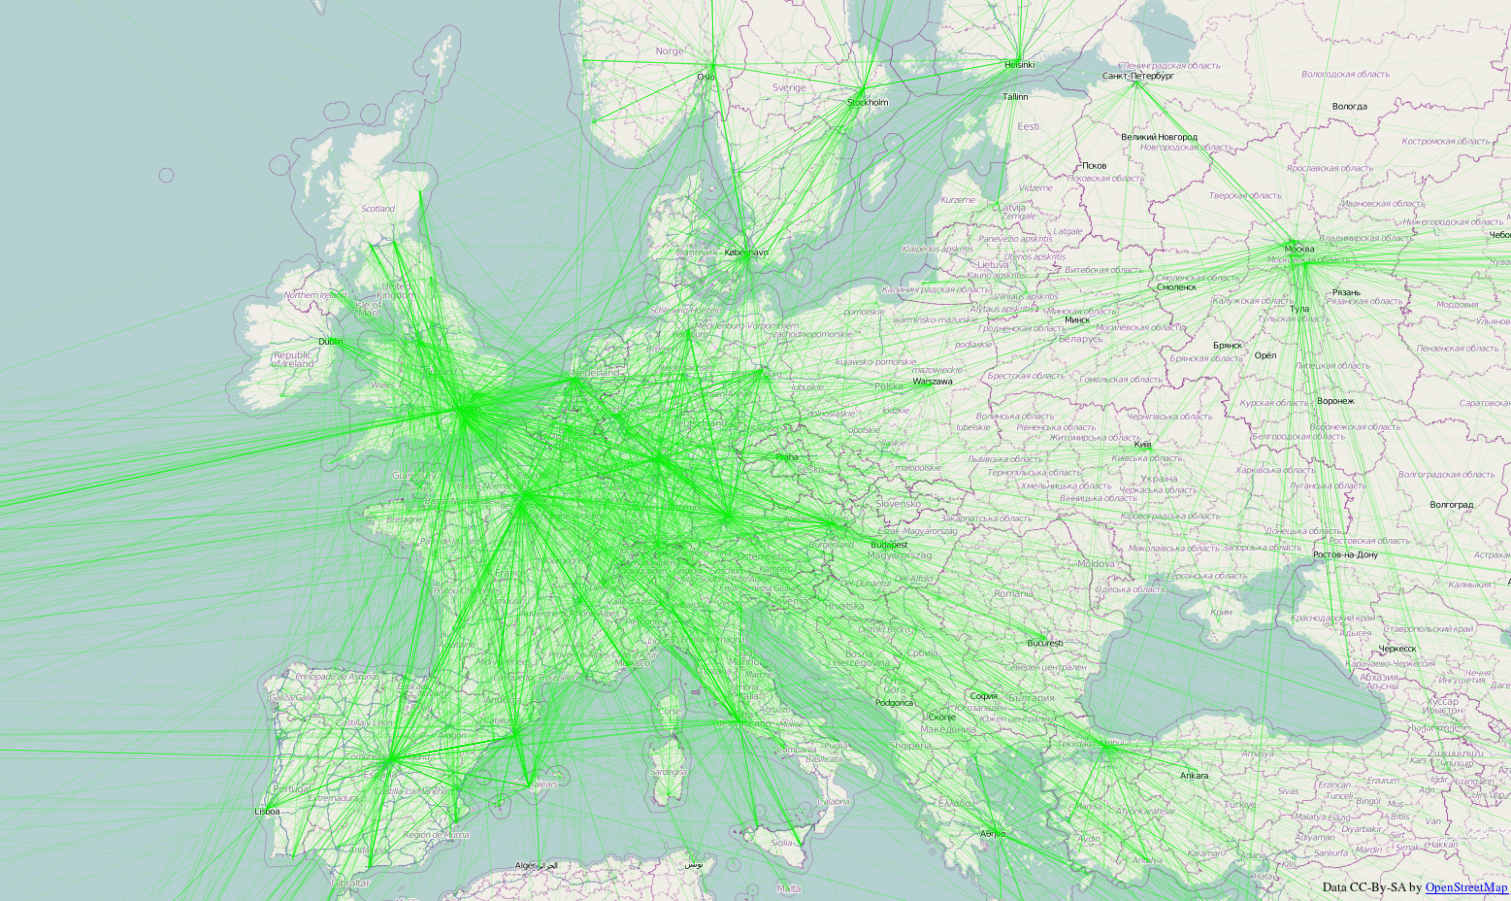
\includegraphics[width=\linewidth]{extending/figures/air/air_network_europe_osm.png}
\end{center}
\caption[European air network]{European air network with country borders in the background (country borders~\textcopyright~\url{openstreetmap.org})}
  \label{fig:matsim_air_network_eu}
\end{figure}

%\subsubsection{Flight Schedule}
%\mnote{Flight Schedule}
The flight schedule is taken from the OAG data and translated to a MATSim Transit Schedule containing information about each line, route, and departure. 
For each airline that offers a connection between two airports, a transit line is generated. 
A transit route, which represents the route on the air traffic network, is created for each flight offered by this airline. 
%The route contains the links belonging to the airport representation plus the specific link for this flight connecting the airports' out- and inbound runway. 
Mutual interferences of aircrafts en-route are not included in the studies presented in this chapter.
%Tab.~\ref{tab:number_of_flights} lists the number of (not included) airports, direct origin-destination (O-D) connections and flight movements for three different area pairs.

%\newcolumntype{R}[1]{>{\hsize=#1\hsize\raggedleft\arraybackslash}X}%
%\newcolumntype{L}[1]{>{\hsize=#1\hsize\raggedright\arraybackslash}X}%
%
%\dissonly{%
%\begin{table}[t]
%	\centering
%	\begin{tabularx}{\linewidth}{L{1.3}R{0.5}R{0.5}R{0.5}R{0.5}R{0.5}R{0.5}}
%%		\hline
%Area pair				& Airports & Airports	missing & O-D Pairs& Flights & Flights missing \\
%\hline
%\\
%Worldwide 		   	& 2333 & 81 & 27496 & 56376 & 2644 \\
%Europe to worldwide & 808		&	16		& 14156					& 21425 & 577\\
%Germany to worldwide & 269	&	3			& 2814	& 4394 & 189 \\
%%\hline
%		\end{tabularx}		
%	\caption{Numbers for different geospatial extents of the model}
%	\label{tab:number_of_flights}
%\end{table}
%}

%\mnote{Time Zones}
%For matters of consistency, all local times are converted into Coordinated Universal Time (UTC). 
%This ensures aircraft taking off and landing at the scheduled times throughout all time zones and also enables the model to reflect incoming and outgoing waves at hub airports worldwide at the appropriate times.

%\subsubsection{Aircraft}

%\mnote{Vehicles}
To represent individual aircraft in the simulation, transit vehicles are created on the basis of OAG data. 
IATA aircraft codes, operating airlines, and seating capacities are reflected in the respective aircraft representation for every flight. 
Information about boarding times, i.e.,\,passenger flow per door over time, is not available, but could be set for each aircraft type. 
One aircraft per flight is generated, thus delays resulting from a delayed incoming aircraft are not modeled.
Accordingly, no aircraft rotations and vehicle trip chains are implemented for the time being. 
The maximum velocity of each aircraft is set to twofold sonic speed, since speed limitations are set for each airway link of the network. 

%\mnote{Results}
%Can be found in \citet{Grether2014PhD}. 
%The results show that the proposed approach can model some important characteristics of air traffic technology.
%In particular, runway capacity restrictions can be added to the model. 


\subsection{Passenger Demand}

%\mnote{Passengers, Synthetic Population}
As soon as you have modeled the technology side of air transport, you can start to simulate a passenger demand. 
The passenger demand for trips in Germany created and used for the results of this section is based on O-D data of DESTATIS 
\footnote{\url{destatis.de}, Fachserie 8 Reihe 6, last access 10.09.2012}. 
Then, for each O-D pair and trip a virtual person is created.
Each virtual person performs two activities, one at the origin and the other at the destination airport. 
Both activities are of same type, thus time spent performing both activities is accumulated before it is evaluated by the utility function according to Section~\ref{sec:charyparnagel}. %equation (\ref{eq:utility_v_perf}). 
A typical duration, $t_{typ,q}$, of $21 \, h$ is set for this activity type. 
The time virtual persons arrive at the origin airport and start waiting for a connection is drawn randomly from a uniform distribution in 04:00 to 18:00, UTC. 
This reflects estimated typical opening hours of airports in Europe.
No other time constraints are set, thus the only incentive for virtual persons is to reduce overall travel time and maximize time spent at the activity. 
In between the two activities a flight leg is scheduled, connecting origin and destination.
As is common, the demand does not specify if a direct flight from O to D is chosen or the virtual person is on a route containing one or more transfers.
The synthetic population contains 51\,832\,virtual persons, 1\,550\,trips from the original data are neglected as origin and destination are equal. 
%

%DESTATIS provides data for passenger movements within Germany in two different representations (referred as data sets 5.1.1 and 5.1.2).
%\footnote{Please note that the table numbers refer to the 2011 version of the DESTATIS data as explained at the beginning of this chapter}. 
%The number of O-D trips between airports is captured in two different ways. 
%
%For all pairs of airports, the number of direct trips between the airports is given in the data set 5.1.1. 
%
%Furthermore, the second data set, 5.1.2, contains O-D pairs that do not include transfers, but the final destination.  %E.g., one person flying from Hamburg (HAM) via Frankfurt (FRA) to Munich (MUC) is contained in the data set 5.1.2 as one O-D pair: HAM $\rightarrow$ MUC.  %The 5.1.1 data counts this person twice, once on the O-D pair HAM $\rightarrow$ FRA and once on FRA $\rightarrow$ MUC.  
%The passenger demand of the second data set, 5.1.2, is used to create the synthetic population. 
%For each O-D pair the number of trips is scaled from monthly to daily values by a division by 30. 
%If the origin or destination airport is available in the simulation model for air transport technology, 
%, otherwise the trip is neglected.
%Both activities are of same type, thus time spent performing both activities is accumulated before it is evaluated by the utility function according to equation (\ref{eq:utility_v_perf}). A \alert{typical duration}, $t_{*}$, of $21 \, h$ is set for this activity type. 
%The time virtual persons arrive at the origin airport and start waiting for a connection is drawn randomly from a uniform distribution in 04:00 to 18:00, UTC. 
%This reflects estimated typical opening hours of airports in Europe.

% ##################################################################################################################
\section{Simulation Results}
\label{sec:air_rail_results}

\subsection{Air Transport}

\mnote{Parameters}
As scenario for air transport technology, a model with Europe to world wide coverage is used. 
Together with the synthetic population it serves as input for the simulation.
%model with no delays and no effective runway capacity restrictions 
%from 
%\technologyCite~is used.
The assignment of concrete flights to the desired O-D connection, i.e.,\,the passenger routing, is calculated by the default public transit routing module of MATSim.

%The routing basically looks for a least cost path in terms of travel time. 
%The graph used for routing is constructed from the information contained in the transit schedule. 
%Each flight is represented by an edge. 
%Transfers are modelled by additional edges, that are implicitly added to the graph. 
%To penalize transfers, the routing assumes an additional cost of $c_{line switch}$ for each transfer edge. 
%The same parameter is also considered by the scoring function, i.e., a (dis-)utility of $-c_{line switch}$ is added to the score of a virtual person for each transfer. 
%The simulation is run several times using different values of the $c_{line switch}$ parameter, i.e., $c_{line switch} \in \{ 0, -6, -12, -18, -24, -30\}/transfer$\footnote{Note, that $c_{line switch}$ cannot be set to values $> 0$ as a standard least cost path calculator cannot handle positive costs for edges.}.  

%\mnote{Simulation Runs}
Each simulation is run for 600\,iterations.
In each iteration, 10\,\% of the virtual persons may shift their departure time randomly within a 2\,hour interval.
Another 10\,\% may seek a new route, i.e.,\,a connection between origin and destination. 
Each passenger choses out of a set of $5$ plans using the multinomial logit model. %(Sec.~\ref{sec:matsim_overview_algo}). 
%The amount of shift is drawn from a uniform distribution.
The outcome is stable after 500\,iterations, thus departure time choice and routing are switched off. 
For another 100\,iterations only the logit model is used by the passengers to select a plan. 
%Empirically, fixing the choice set for the last 100~iterations reduces the noise of learning and eases analysis and intepretation of results. 

%\mnote{Computation Time}
%One iteration takes around~$5 \, min$~on an Intel Xeon Processor ($2.67 \, GHz$) using one core for the execution of mobility simulation and two cores for the replanning modules. 
%Overall computation time for one simulation run is roughly 2 days.  


%\subsection{Results -- Remove}
%
%\begin{figure}[t]
%		\centering
%		\begin{subfigure}[t]{0.45\textwidth}
%			\centering
%			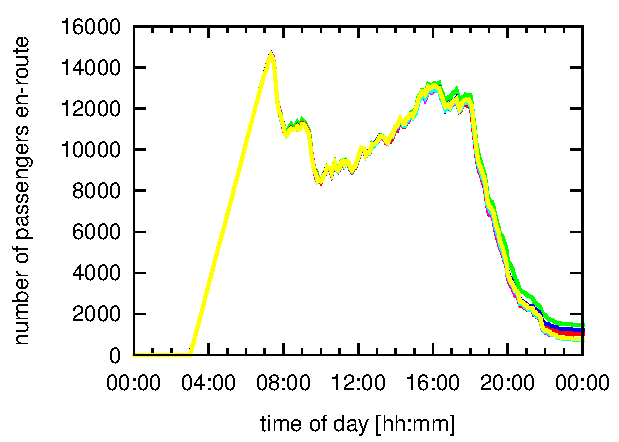
\includegraphics[width=\textwidth]{./extending/figures/air/leg_histogram_flight_pt_en-route_1876-1881_it_0.pdf}
%			\caption{After 0th iteration}
%			\label{fig:2009_demand_it0}
%		\end{subfigure}
%		\begin{subfigure}[t]{0.45\textwidth}
%			\centering
%			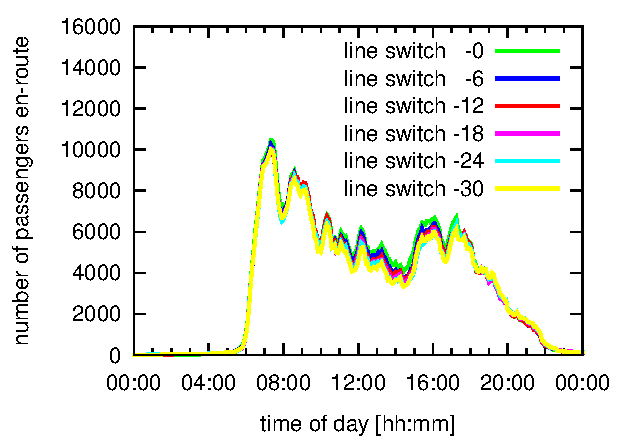
\includegraphics[width=\textwidth]{./extending/figures/air/leg_histogram_flight_pt_en-route_1876-1881_it_600.pdf}
%			\caption{After 600th iteration} %run1836ff it 600
%			\label{fig:2009_demand_it600}
%		\end{subfigure}
%	\caption{Passengers waiting for a flight or traveling by plane over time of day}
%\end{figure}
%
%\mnote{Zeroth Iteration}
%First, to show the effects of routing, the result after the zeroth simulated iteration is presented. 
%Each virtual person gets a connection assigned based on a generalized cost routing for the connection and the preset departure time.
%Fig~\ref{fig:2009_demand_it0} shows the number of travelers en-route, i.e., waiting for a flight or traveling by plane, as a function of the time-of-day.
%Some passengers are still waiting for a flight at midnight.
%As only one day of operation is simulated, these passengers are stuck and will not reach their destination.
%The number of these \alert{stuck} passengers is decreasing with the increasing disutility of line switch.
%
%\mnote{Iteration 600}
%The output after 600~iterations is depicted in Fig.~\ref{fig:2009_demand_it600}. 
%The shape of all curves is different from the shape of the zeroth iteration. 
%One can identify two morning and two evening peaks.
%Some passengers still get stuck at the end of the day, but fewer than in the 0th iteration.
%In addition, the influence of the $c_{lineswitch}$ parameter is diminishing in respect to the stuck passengers.
%
%\mnote{Error Calculations}
%grether2014phd
%To study the influence of the $c_{lineswitch}$ parameter, the simulation results are compared with the input data. 
%Recall, that the synthetic population is generated based on O-D pairs that may contain transfers ($od_{transfers}$), 
%while other data directly counts the number of passengers on actual direct flights ($od_{direct}$). % (2.2.1).
%The latter is used to evaluate the accuracy of the model.
%For comparison, the number of passengers on direct flights is calculated for each O-D pair ($sim_{direct}$) from the simulation results.
%
%Based on these data sets, the mean square error $\sigma^2$ is computed as
%\begin{equation*}
%	\sigma^2 = \frac{\sum_{i \in OD} (sim_{direct}(i) - od_{direct}(i))^2}{|OD|} \, , 
%\end{equation*}
%whereby $|OD|$ denotes the number of O-D pairs, $sim_{direct}(i)$ the simulated passengers on a direct flight between the O-D pair $i$, and $od_{direct}(i)$ the same, but retrieved from data.  
%With the same values, the (unsigned) mean relative error for each O-D relation is calculated as
%$$
%\mbox{mean rel error} = \frac{\sum_{i \in OD} |(sim_{direct}(i) - od_{direct}(i))|/ od_{direct}(i)}{|OD|}.
%$$

%\mnote{Results}
%The first line contains the comparison of the two sets of input data from DESTATIS, i.e., in the above formulas, $sim_{direct}$ is replaced by $od_{transfers}$. 
%This serves as reference as it would assume that \alert{all} demand is served by direct flights.
%All simulation runs explain the data better than that reference.
%Mean square error, variance, and number of stuck passengers increase with decreasing values of $c_{lineswitch}$. 
%The relative error, however, decreases. 
%So far, variance and relative error are hard to interpret, as they point in opposite directions. 
%First, the reasons for stuck passengers are analyzed in detail. 

%\begin{table}[h!]
%\centering
%		\begin{tabular}{@{}l|ccccc@{}}
%			$c_{lineswitch}$ & $\sigma^2$ & $\sigma$ & mean rel error  & stuck \\
%\hline
%$od_{transfer} - od_{direct}$ & 12640 & 112 & 1.75 & - \\
%\\
% -0  	 & 9293 & 96 & 0.36		& 320 \\	%	1876 & 600 
% -6  	 & 9878 & 99 & 0.35		& 338 \\  %  1877 & 600
% -12 	 & 10361 & 102 & 0.33 & 350 \\%  1878 & 600
% -18 	 & 10552 & 103 & 0.32 & 378 \\%  1879 & 600
% -24 	 & 10916 & 104 & 0.32 & 373 \\%  1880 & 600
% -30 	 & 11090 & 105 & 0.32 & 386 \\%  1881 & 600
%		\end{tabular}
%		\caption{Simulation results for different values of $c_{lineswitch}$, iteration 600}
%		\label{tab:2009_results_line_switch}
%\end{table}

\begin{figure}[t]
	\centering
	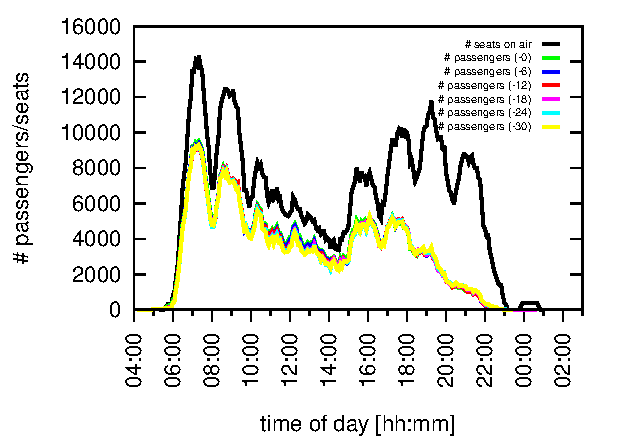
\includegraphics[width=0.9\linewidth]{./extending/figures/air/in_vehicle_histogram_flight_1876-1881_it_600.pdf}
	\caption{Passengers in aircraft and available seats over time in Germany, iteration 600}
	\label{fig:2009_passengers_seats}
\end{figure}

Results are then taken from the output of the 600th iteration. 
Filtered by flights in Germany, Figure~\ref{fig:2009_passengers_seats} depicts passengers in aircraft and seats therein over time of day. 
Some passengers fail to reach their destination, they get stuck.   
This is considered unrealistic, as only trips within Germany are modeled, which are usually completed within a few hours without any requirement for an overnight stay at an airport. 
%Tab.~\ref{tab:2009_results_line_switch} shows the results for these calculations. 
320\,passengers get stuck at the end of the day. %, but fewer than in the 0th iteration.
Getting stuck is not a consequence of a general lack of seats: at any time of day, there are more seats than demand.  
%
There are many reasons why stuck passengers can arise in such a situation.
%
Further analysis of the simulation results leads to the following insights for the $c_{lineswitch} = 0$ scenario:
\begin{itemize}

\item 92\,passengers are stuck because there is no seat, and there is no other flight by the same airline later during the day to which they would be shifted otherwise.

\item 228\,passengers are stuck at an airport because there is no connection after their departure time 
	between that airport and their destination airport. 
\end{itemize}

Figure~\ref{fig:2009_passengers_seats} further reveals the tendency of passengers to depart early. 
Neither getting stuck nor departing early are behavioral aspects explicitly modeled.  

%\begin{figure}[t]
%	\centering
%	\subcaptionbox{Passengers in aircraft and available seats over time in Germany, iteration 600\label{fig:2009_passengers_seats}}[0.49\linewidth][l]{
%	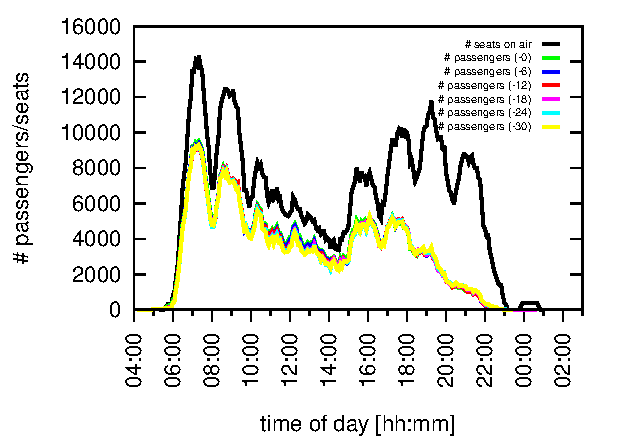
\includegraphics[width=0.48\linewidth]{./extending/figures/air/in_vehicle_histogram_flight_1876-1881_it_600.pdf}
%	}
%	\subcaptionbox{Correlation between the available seats, the demand for seats ($od_{transfer}$) and the number of passengers being stuck, iteration 600\label{fig:2009_seats_demand_stuck}}[0.49\linewidth][l]{
%	\includegraphics[width=0.48\linewidth]{./extending/figures/air/1876_demand_seats_stuck.pdf} 	
%	}
%	\caption{Potential reasons for stuck passengers}
%\end{figure}

%\mnote{Departure Time}
%To study the influence of departure time on available connections, several simulations are run that set the departure time of each passenger being stuck to 04:00 UTC, i.e., before the first aircraft is departing. 
%Simulation results produced similar findings as presented above. 

%\mnote{Demand \& Seats}
%Thus, it is worth looking more closely at the relation between passengers being stuck and the capacity of seats offered for each O-D pair. 
%For each O-D pair, one can obtain the number of travelers that plan to travel from O to D, i.e., the number of virtual persons, $od_{transfer}$ (data set 5.1.1). 
%Further, the number of seats offered on that O-D pair can be retrieved from simulation input data. 
%Fig.~\ref{fig:2009_seats_demand_stuck} plots the number of travelers that are stuck on their planned O-D connection over the difference between seats and $od_{transfer}$. 
%To improve visibility the figure %Fig.~\ref{fig:2009_seats_demand_stuck} 
%is cut at values where available seats increase demand by more than 800 --- the number of stuck persons is always 0. 
%Apparently, passengers get more likely stuck the more the requested demand is equal or greater than overall capacity. 


\subsection{Adding an Alternative Mode}

%\mnote{Simulation Setup}
To gain further insights, in the following a slightly different simulation setup is applied. 
%The additional cost for each transfer is fixed to $c_{lineswitch} = 0$ and has no influence on the model. 
A second option for mode choice is added. 
Each virtual person can now choose between the micro-simulated air transport options and an alternative mode. 
The alternative mode has no capacity restrictions. 
Furthermore, passengers that travel with the alternative mode can start directly at their randomly selected departure time. 
The travel time, $tt$, is computed by the microsimulation with an estimation of the beeline distance between the O-D pair $d$ and a velocity $v$, i.e.,\,$tt = d / v$.  
This velocity is varied in several simulation runs, i.e.,\,$v \in \{100, 150, 200, 250, 300 \} [km/h]$. 
If the alternative mode is chosen, the (dis-)utilities for traveling in the scoring are calculated accordingly.  

%Each person in the synthetic population obtains a second plan that uses the alternative mode. 
With this population the simulation is again run for 600\,iterations. 
Like in the previous simulations 10\,\% of the virtual persons may shift their departure times while another 10\,\% seek a different route between origin and destination in the air transport network. 
Additionally, further 10\,\% of virtual persons may change mode, i.e.,\,they can switch between the air traffic mode and the alternative mode. 
After 500\,iterations all choice modules are switched off, thus for the last 100\,iterations the logit model is used by passengers to select one of their plans. 

Simulation results for the 600th iteration show that the 
%, the same numbers as for the previous simulation runs are calculated (Tab.~\ref{tab:2009_results_alternative_mode}). 
increasing speed of the alternative mode affects the modal split. % (Tab.~\ref{tab:2009_results_train_modal_split}).  
While for a $v = 100 \, km/h$ the alternative mode is chosen by 1.2\,\% of the passengers, a mode alternative with a speed of $300 \, km/h$ attracts 15.69\,\% of travelers. 
The number of stuck passengers for the alternative mode with $v = 100 \, km/h$ is remarkably reduced from approx.~$320$ to $67$. 
Higher speeds of the alternative mode further reduce the number of stuck passengers. 
Slow speeds of the alternative mode implicate a dominance of the air transport mode. 
If there is a seat on a flight, travelers receive a higher score than by traveling on the alternative mode. 
However, travelers risk to get stuck, which can be hard to analyze and interpret. 
Further, it is an open issue of the implemented algorithm: If the number of plans per traveler exceeds a threshold of $5$ the plan with the lowest score is removed from the . 


%Both error values increase. 
%As passengers no longer get stuck, the model seems more plausible, but deviates from the given data. 

%If the speed of the alternative mode is $100$ or $150 \, km/h$ mean square and relative error are quite similar to the previous results.  

%\begin{table}[t]
%\centering
%		\begin{tabular}{@{}l|ccccc@{}}
%			$v [km/h]$ & $\sigma^2$ & $\sigma$ & mean rel error  & stuck \\
%\hline
%$od_{transfer} - od_{direct}$ &  12640 & 112 & 1.75 &  - \\
%\\
%100	& 9388 & 97 & 0.37   &  67 \\	% 1903 & 600
%150	& 9911 & 100 & 0.35  &  50 \\	% 1904 & 600
%200 & 12075 & 110 & 0.37 &  6 \\	% 1905 & 600
%250 & 13759 & 117 & 0.39 &  0 \\	% 1906 & 600
%300 & 13790 & 117 & 0.42 &  0 \\	% 1907 & 600
%		\end{tabular}
%		\caption{Simulation results including an alternative mode at different speeds $v$}
%		\label{tab:2009_results_alternative_mode}
%\end{table}


%\begin{table}[t]
%\centering
%		\begin{tabular}{@{}l|ccc|ccc@{}}
%$v [km/h]$	& \# air mode  & \# alt.~mode & \# stuck & air mode[\%]  & alt.~mode[\%] & stuck[\%] \\
%\hline 
%100	& 51143 & 622 & 67 & 98.67 & 01.20 & 00.13\\	%1903 & 600 51832
%150	& 50213 & 1569 & 50& 96.88 & 03.03 & 00.10\\	%1904 & 600 51832
%200 & 48541 & 3285 & 6 & 93.65 & 06.34 & 00.01\\	%1905 & 600 51832
%250 & 46748 & 5084 & 0 & 90.19 & 09.81 & 00.00\\	%1906 & 600 51832
%300 & 43698 & 8134 & 0 & 84.31 & 15.69 & 00.00\\	%1907 & 600 51832
%		\end{tabular}
%		\caption{Modal split for different speeds of the alternative mode, iteration 600}
%		\label{tab:2009_results_train_modal_split}
%\end{table}
%
%
%\begin{figure}[t]
%	\centering
%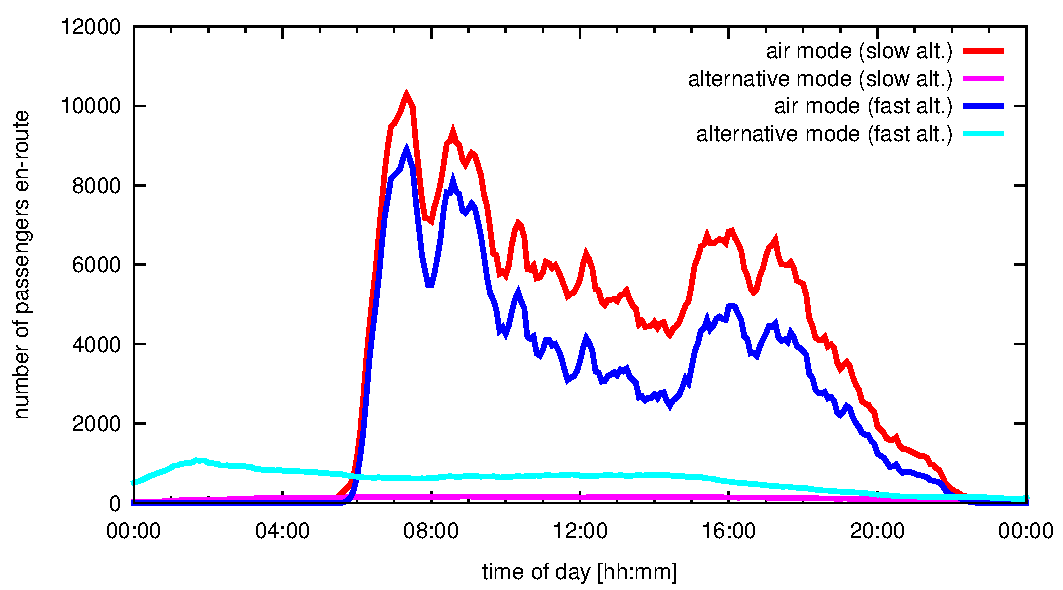
\includegraphics[width=\linewidth]{./extending/figures/air/leg_histogram_improved_flight_train_en_route_1903_1907_it_600.pdf}
%	\caption{Passengers waiting for a flight or traveling by plane or by the alternative mode over time of day, iteration 600}
%	\label{fig:2009_leg_histogram_modes}
%\end{figure}


%Fig.~\ref{fig:2009_leg_histogram_modes} illustrates temporal effects for the alternative mode at speeds of $100 \, km/h$ and $300 \, km/h$. 
%One can observe that passengers using air transport follow the time distribution of the offered capacity.  
%In contrast, travelers on the alternative mode are spread over time of day. 
%This is plausible considering the setup of simulation: Passengers have no time constraints that force them to arrive at a certain time at their destination. 
%Departure times are equally distributed between 04:00 and 18:00, UTC, and then randomly mutated during the iterations. 
%As the alternative mode is always available there is no constraint within the model that ties passengers to any departure time. 

%\mnote{Black Box?}
%One might conclude with these results. 
%A more accurate inspection of the results, however, raises the question why travelers on both modes have a tendency to depart early in the morning. 
%Furthermore, if a not capacity constrained alternative is available, one might wonder why travelers prefer to get stuck instead of traveling on the alternative mode.
%One can reveal further insights by a closer look at the implemented algorithm. 
%
%\mnote{Time Choice}
%The public transit used for the simulation runs boards passengers to transit vehicles in order of appearance at the transit stop. 
%If the passenger capacity of the vehicle is reached, passengers can no longer board. 
%If there is passenger capacity available in a subsequent transit vehicle of the same line, passengers may board this vehicle~\citep[][p.~67]{Rieser2010}. 
%For the air transport model, this implies that the earlier travelers arrive at the airport, the higher is the probability they get a seat. 
%This explains the passengers' tendency towards earlier flights, even though the modeling is not specifying any constraints that justify this behavior. 
%To understand the shift towards earlier departures in case of the alternative mode, a closer look at the mode choice model is required. 

%\mnote{Mode Choice}
%The mode choice model tested and validated in~\citep{RieserGretherNagel2008modeChoiceCalculations} specified a constraint for the plan database: 
%Only one mode can be set for each plan. 
%At least one plan of every mode is kept in the plan database of every virtual person. 
%This constraint was removed in further studies, motivated by the need of more complex plans. 
%In the current version, each leg between two activities can have a different mode. 
%The mode of each leg is then varied randomly over the iterations~\citep[][p.~77]{Rieser2010}. 

%\mnote{Implications}
%Aware of these changes, one can now explain why travelers get stuck even if there is an alternative. 
%Slow speeds of the alternative mode implicate a dominance of the air transport mode. 
%If there is a seat on a flight, travelers receive a higher score than by traveling on the alternative mode. 
%For the first $500$ iterations, some virtual persons try different routes, times, or modes. 
%Thus, during this phase a certain amount of seats is not occupied. 
%More virtual persons validate the air mode as good choice than there are available seats. 
%The corresponding plans get a higher score than the plans for the alternative mode and shift towards earlier departure times. 
%Recall, that the plan with the lowest score is deleted when the number of plans excesses a certain threshold (Sec.~\ref{sec:matsim_overview_algo}). 
%For the first $500$ iterations, this is the plan for the alternative mode. 
%If plans for the alternative mode are recreated, they are copied from an air mode plan and obtain its departure time. 
%Then, choice dimensions are switched off. 
%Only the logit model is used for selection of existing plans. 
%Travelers, that have tried the alternative mode in the previous iteration, switch back to the air transport mode with a high probability. 
%This results in a lack of seats that are then allocated by time of arrival. 
%Passengers rejected to board their flight get stuck. 
%The probability to avoid getting stuck is higher the earlier one arrives at the airport. 
%As the plan for the alternative mode is deleted before air transport plans, in most cases the plan database of a virtual person no longer contains this option. 
%Otherwise, passengers may switch to the alternative mode with a tendency towards an early departure. 

%\mnote{Potential Solution, Stuck}
%This analysis reveals several problems to be solved in the overall simulation process before air transport specific questions can be addressed further. 
%In the following, a potential solution is presented that prevents passengers to get stuck. 
%Theoretically, one could increase the threshold for the maximum number of plans per person to infinity.
%In practice, this is not feasible, as memory is limited. 
%The solution used for the study in~\citep{RieserGretherNagel2008modeChoiceCalculations} cannot be applied to more complex plans. 
%Some more complex heuristic is required to measure the similarity of plans. 
%This heuristic can be implemented by a functionality similar to the path size logit formulation~\citep[e.g.][]{FrejingerBierlaire2007PathSizeLogit}. 
%That is, a score penalty, $\beta_{PS} \cdot \ln{PS_{in}}$, can be added to a plan when it is similar to other plans, whereby $\beta_{PS}$	is a scale parameter and $PS_{in}$ measures similarity by
%\[
%PS_{in} = \sum_{a \in \Gamma_i} \frac{l_a}{L_i} \frac{1}{\sum_{j \in C_n} \delta_{aj}} \, ,
%\]
%whereby $\Gamma_i$ is the set of legs in plan $i$, $C_n$ the set of plans of person $n$, and $\delta_{aj}$ the overlap function.
%$\delta_{aj}$ equals $1$ if leg $a$ is contained in plan $j$ and $0$ otherwise\footnote{
%A leg for the air transport mode is already contained in the plan database if transit line and route are equal.
%Legs of the alternative mode are considered equal, if they connect the same activity locations by equal travel times. 
%Note, that this implementation may be subject to change. 
%}. 
%The scheduled travel time of leg $a$ is $l_a$, and $L_i$ denotes the sum of all scheduled travel times of plan $i$. 
%
%Then, instead of removing the plan with the lowest score, the plan $i$ of a virtual person $n$ for deletion is selected randomly with probability 
%\[
%p(i) \; \propto \; e^{-\mu (V_i + \beta_{PS}\ln{PS_{in}})} \, ,
%\]
%where $V_i$ is the score, $\mu$ the sensitivity parameter from Eq.~\ref{eq:UtilityFunction}, and $\beta_{PS}$, $PS_{in}$ denote the same as above.  

%\mnote{Results}

\begin{figure}[t]
	\centering
	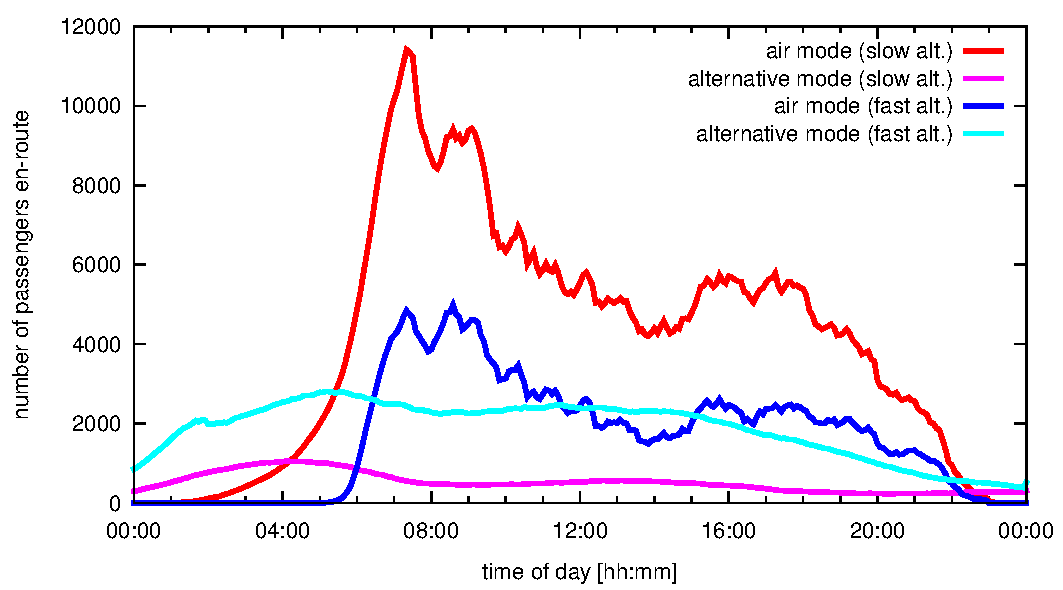
\includegraphics[width=\linewidth]{./extending/figures/air/leg_histogram_improved_flight_train_en_route_1893_1897_it_600.pdf}
	\caption{Results with random selector for plan removal, iteration 600. Passengers waiting for a flight or traveling by plane or by the alternative mode over time of day}
	\label{fig:2009_leg_histogram_modes_psl}
\end{figure}

\begin{table}[t]
	\centering
	\begin{tabular}{@{}l|ccc|ccc@{}}
		$v [km/h]$	& \# air mode  & \# alt.~mode & \# stuck & air mode[\%]  & alt.~mode[\%] & stuck[\%] \\
		\hline 
		100 & 49280 & 2551 & 1 & 95.08 & 04.92 & 00.00\\	%1893 & 600
		150 & 44835 & 6996 & 1 & 86.50 & 13.50 & 00.00\\	%1894 & 600
		200 & 39929 & 11902 & 1 & 77.04 & 22.96 & 00.00\\	%1895 & 600
		250 & 34332 & 17499 & 1 & 66.24 & 33.76 & 00.00\\	%1896 & 600
		300 & 27270 & 24562 & 0 & 52.61 & 47.39 & 00.00\\	%1897 & 600
	\end{tabular}
	\caption{Results with random selector for plan removal, iteration 600. Modal split for different speeds of the alternative mode}
	\label{tab:2009_results_train_modal_split_psl}
\end{table}

Instead this deterministic removal of plans a probabilistic algorithm can be implemented, e.g.,\,plans for removal can be selected based on a path size logit model. 
With this modification the simulation runs are repeated. 
%with the same setup as for the runs that includes the alternative mode. 
Figure~\ref{fig:2009_leg_histogram_modes_psl} shows the resulting travel patterns over time for alternative modes at speed 100\,km/h and 300\,km/h.  
The distribution of travelers on the alternative mode over time of day is quite homogeneously. 
The speed increase of the alternative mode attracts more passengers. 
This is reflected by the modal splits in Table~\ref{tab:2009_results_train_modal_split_psl}. 
Only one passenger gets stuck at the end of day. 

\begin{table}[t]
\centering
		\begin{tabular}{@{}l|ccccc@{}}
			$v [km/h]$ & $\sigma^2$ & $\sigma$ & mean rel error  & stuck \\
\hline
 $od_{transfer} - od_{direct}$ &  12640 & 112 & 1.75 & - \\
 \\
 100	& 10367 & 102 & %\colorbox{markergreen}{
 0.35%} 
 &  %\colorbox{markergreen}{
 1
 %} 
 \\	% 1893 & 600
 150	& 13820 & 118 & 0.43 &  1 \\	% 1894 & 600
 200 & 18651 & 137 & 0.56 &  1 \\	% 1895 & 600
 250 & 25291 & 159 & 0.68 & 1 \\	% 1896 & 600
 300 & 36059 & 190 & 0.76 & 0 \\	% 1897 & 600
		\end{tabular}
		\caption{Results with random selector for plan removal, iteration 600. Simulation results including an alternative mode at different speeds $v$}
		\label{tab:2009_results_alternative_mode_psl}
\end{table}

The simulation results are further compared with the data of DESTATIS that serves as basis for the virtual population.  
The synthetic population is generated based on O-D pairs that may contain transfers ($od_{transfers}$), 
while other DESTATIS data directly counts the number of passengers on actual direct flights ($od_{direct}$). % (2.2.1).
The latter is used to evaluate the accuracy of the model.
For comparison, the number of passengers on direct flights is calculated for each O-D pair ($sim_{direct}$) from the simulation results.
Based on these data sets, the mean square error and the mean relative error are calculated\footnote{
The mean square error $\sigma^2$ is computed as
	$\sigma^2 = \frac{\sum_{i \in OD} (sim_{direct}(i) - od_{direct}(i))^2}{|OD|} \, , $
whereby $|OD|$ denotes the number of O-D pairs, $sim_{direct}(i)$ the simulated passengers on a direct flight between the O-D pair $i$, and $od_{direct}(i)$ the same, but retrieved from data.  
With the same values, the (unsigned) mean relative error for each O-D relation is calculated as
$
\mbox{mean rel error} = \frac{\sum_{i \in OD} |(sim_{direct}(i) - od_{direct}(i))|/ od_{direct}(i)}{|OD|}.
$
}

Table~\ref{tab:2009_results_alternative_mode_psl} shows the outcome of these calculations. 
The first line contains the comparison of two sets of input data from DESTATIS\footnote{In the calculation, $sim_{direct}$ is replaced by $od_{transfers}$.}. 
This serves as reference as it would assume that all demand is served by direct flights.
All simulation runs explain the data better than that reference.
Mean square error and variance increase with the speed $v$ of the alternative mode.  
This is plausible as the demand only covers air transport trips. 
%The mean square error is higher than without the alternative mode. 
%(Tab.~\ref{tab:2009_results_alternative_mode_psl}). 


\section{Interpretation \& Discussion}
\label{sec:air_rail_discussion}
%\subsection{Alternative Mode}

%\mnote{Interpretation}
The alternative mode can be interpreted as mixture between train, bus, or car connection availability. 
Clearly, the results hinge at the assumption that the alternative mode is always available and not capacity restricted.  
All passengers on the alternative mode face the same travel speed. 
This assumption is too coarse for the presented scenario. 
E.g., average speed and temporal availability of train connections depends on the O-D pair. 
In principle, the alternative mode could be refined by inclusion of O-D pair dependent average speed data. 
Alternatively, train, bus, and car can be simulated explicitly, featuring capacity restrictions and mutual interactions. 
For illustration of the overall modeling approach, however, a homogeneous velocity for the alternative mode seems to be more appropriate. 
%\mnote{Effects}
The effects evoked by the availability of the alternative mode are illustrative. 
%Interpretation of the effects by the availability of the alternative mode must be undertaken with care. 
The data for the demand provides O-D pairs for air transport, but not for car, train or bus trips.  
%Thus, the simulation results should get worse when the alternative mode is added. 
%This is reflected by the presented results. 
For more plausible interpretations, further data for demand on other modes is required. 
%Alternatively, the 2011 data could be used. 


%\subsection{Overall Approach}

%\mnote{Extent}
All the presented modeling approaches explain the routing of passengers in more detail than it can be solely retrieved from the input data.  
Most passengers use a direct connection, which is highly plausible considering the geospatial extent of the demand.  
Flying within Germany is often not worth it, if the connection includes a transfer. 
Then, empirically it is faster to travel by train, car, or bus. 
To gain further insights, the geospatial extent of the modeled demand could be increased which hinges at the availability of data not on the overall simulation approach. 
%Data for all Europe is still hard to collect.  

%\mnote{Time Structure}
Passengers are modeled without explicit desired departure or arrival times. 
The input data for this study does not contain any information about time distribution. 
The simulation approach can capture such individual time constraints.  
With some more data, the information can be added without big effort. 
This would resolve some of the presented problems concerning departure time choice. 
%A detailed modeling of individual time constraints is not considered in this study. 

%\subsection{Air Transport Only}
%
%\mnote{Stuck}
Passengers getting stuck are considered as not desired artifact of the simulation. 
Without the alternative mode, the only available transport mode is a capacity restricted flight connection that is served in discrete, irregular time intervals. 
The number of stuck passengers is higher than for the simulation runs with the alternative mode. 
Passengers get more likely stuck on O-D pairs where the demand excesses seat capacity. 
This may have model extrinsic and intrinsic reasons. 

%\mnote{Extrinsic Stuck}
%Choice, quality, and preprocessing of available data sources is extrinsic.  
The quality of the simulation model's outcome hinges at the data available.  
For older studies of the air transport passenger demand, DESTATIS data for 09-2011 were used
%\footnote{
%For some reason, DESTATIS provides historical data up to 01-2010. 
%Older data is not available. 
%Special thanks to Dr.~Tobias Grosche for providing the 2009 DESTATIS data.  
%}. 
The air transport technology model, however, was created on a 09-2009 flight schedule.  
The number of starts of flights within Germany increased slightly between 2009 and 2011~\citep[][p.~23]{DLR2011Luftverkehrsbericht}. 
Assuming that the number of available seats is increased accordingly, the simulation model provided too little capacity, at least on certain O-D pairs. 
As result, the number of passengers that had not reached their destination but got stuck was much higher. 
%These results can be found in Appendix~\ref{app:chpt:air_2011}. 
With the availability of 09-2009 DESTATIS data, the overall quality of results increased.  
The replacement of the 2011 data by 2009 data reduced the number of stuck passenger significantly, from around 1500 to 350\,travelers. 

Data is provided on a monthly basis, while the time horizon of the simulation model is one day. 
The number of trips per day is retrieved on the assumption that trips are uniformly distributed over all days of a month.  
The remaining 350\,stuck passengers might be resolved by a more accurate distribution. 
Otherwise, a longer time horizon could be simulated\footnote{Note, that this requires some changes in the source code that may not be resolved by sole customizations of MATSim. Please ask the developers before running MATSim for a longer time horizon.}. 
This would also include flights that are not departing on a Tuesday. 
Possibly, travelers no longer get stuck. 

%\mnote{Intrinsic Stuck}
The problem of stuck passenger can be model-intrinsic. 
The algorithm that removes plans is apparently the pivotal point to avoid stuck passengers. 
Replacement of the deterministic by a probabilistic formulation resolves most of the stuck passengers. 
The applied path size logit modeling approach seems to be feasible, but requires further studies for parametrization and interpretation. 
In general, it allows the generation of more heterogeneous choice sets, see also Section~\ref{sec:choicesets}. 
With the deterministic plan removal plans with a high score but similar structure dominate all other generated plans.In combination with capacity restrictions the lack of alternatives results in stuck passengers.  
All other approaches to simulate more heterogeneity discussed on the following should consider these effects.  

%\mnote{Time Structure and Prices}
In further studies departure time choice and cost structures can be refined. 
If there is only one, early, connection to a hub per day, departure times of some passengers might be too late to reach that connection. 
The random departure time mutation may not be able to find that connection for all passengers. 
This has been ruled out for the current setup but should be considered in further studies. 

Alternatively, it may be the case that passengers have a connection that works in theory, but they are ``crowded out'' by other passengers who arrive earlier at the gate.  
They would make it if either of them would take a different route.  
The current approach would not find such a solution, since passengers do not take into account the costs they impose on others, see~\citet{LaemmelFloetteroed2009KISysOptEvac} for an approach to take that into account.  
The real-world solution presumably would be to raise prices on congested seats until one or the other passenger re-routes. 
Currently, all passengers have homogeneous values of time.   
For a more meaningful price modeling, more heterogeneous attributes of passengers can be included. 
As the present model is based on sole O-D data, it does not include such a process. 
In principle, other data, as e.g.~Lorenz curves and median incomes, can be merged with the O-D data~\citep{KickhoeferEtAl2011PolicyEvaluationIncome}.  

%\mnote{Diversity Routing}
An alternative approach to improve heterogeneity is a router that generates a larger diversity of routes even for the same departure time.  
Such a router would be able to point a passenger to a route where seats are available without by itself knowing about seat availability.  
That approach would, however, not address the issue that some passengers might need to switch their path in order to allow others to obtain a feasible path. 
In~\citet{Graf2013Da}, a first prototype of such a router is tested in a different context. 
First tests for the flight model revealed only slight improvements. 
As more diverse routes are dominated by the direct connection, they are removed by the algorithm similar to routes on slow alternative modes. 
After this more general problem is solved, a more diverse routing should be reconsidered. 

\section{Conclusion}

Overall, the results show that a microscopic, agent-based simulation of passenger demand for air transport is feasible. 
Most passengers are able to learn the constraints of air transport technology and arrive at their desired destination.

%Despite the lack of detail, some relevant aspects of congestion and delays can be captured by a queue model for traffic flow.
%The queue model is computationally relatively cheap so large scenarios can be simulated.
%As proof of example results for the Europe to world air transport are presented.
The modeling of technology is similar to the approach by~\citet{ClarkeEtAl2007AirNetworkSim}, the level of detail is, however, coarser. 
In the same way as~\citet{ClarkeEtAl2007AirNetworkSim}, further models for, e.g., gates, taxiing, weather or airline operations can be added to the presented approach. 
As the open source code of MATSim comes with options for extension, more detailed models of the technology side hinge on the availability of data. 
In contrast, and going beyond~\citet{ClarkeEtAl2007AirNetworkSim}, passengers are captured at all stages of their trip. 
Further, passengers traveling on alternative transport modes can be simulated. 
The chapter discusses some open issues, that are considered more general and not specific to air transport systems. 
The advice to the interested user is to support the MATSim team in solving these more general questions first.  
Then, the model may help to get a more detailed picture of mid-distance travel patterns.

%\mnote{Potential Applications}
Clearly, potential applications of the proposed model depend on type and detail of included information. 
In general, application for policy planning allows a more detailed evaluation of the effects from mid-distance travel policies that includes consideration of mode alternatives. 
The approach could also be useful for private companies, planning flight-schedules and capacities on different connections. 
The impacts of changes on customers can be assessed on a high level of detail. 

%\mnote{Technology}
%In the first part of this chapter, a microscopic modeling approach for air transport technology is presented.  
%A multi-agent simulation, originally developed for urban transport planning and forecasting, is used. 
%Aircraft are represented microscopically, featuring attributes as speed, available seats, and boarding constraints. 
%The air traffic network and flight performance is captured at a low level of detail as air traffic management applications are not intended. 
%Despite the lack of detail, some relevant aspects of congestion and delays can be captured by a queue model for traffic flow.
%The queue model is computationally relatively cheap so large scenarios can be simulated.
%As proof of example results for the Europe to world air transport are presented.
%Overall modeling of technology is similar to the approach by~\citet{ClarkeEtAl2007AirNetworkSim}, the level of detail is, however, coarser. 
%In principle, in the same way as~\citet{ClarkeEtAl2007AirNetworkSim}, further models for, e.g., gates, taxiing, weather or airline operations could be added to the presented approach. 
%In contrast, and going beyond~\citet{ClarkeEtAl2007AirNetworkSim}, passengers are captured at all stages of their trip. 
%Further, passengers traveling on alternative transport modes can be simulated. 
%
%\mnote{Passengers}
%An agent-based modeling of passengers is subject of the second part of this chapter. 
%For this, a passenger demand for the German national air transport system is set up. 
%The computationally affordable simulation technique enables an iterative, simulation-based assignment of passengers to flights of the Europe to world wide model for air transport technology. 
%Furthermore, alternative transport modes can be added. 
%Overall, the presented results look promising. 
%Some problems of the overall simulation technique are uncovered. 
%These are more general and not specific to air transport systems. 
%Several solutions are presented and discussed. 
%Potentially, the overall problem can be solved with some of them. 
%Further research, however, is required before the passenger model can be refined and calibrated. 
%Then, the model may help to get a more detailed picture of mid-distance travel patterns.
